\documentclass[a4paper]{article}
\usepackage{import}
\subimport{../}{preamble}
\begin{document}

\section{Quantum Effects in Sub-nm Gaps between Spherical-Tipped AFM Probes}
% atomic structure and mention of direct above-barrier transmission \cite{barbry2015}
% qcm transmission correlated with blueshift screening \cite{esteban2015}
% nonlocal smooths sharp edges reducing the ability to excite higher order modes, smoothening spectral trends and preventing unphysical divergences. Tunnelling neutralises opposite charge accumulation on gap surfaces.

Should the surfaces of two approaching spherical surfaces be sufficiently clean that the formation of a sub-nm gap becomes possible, the influence of quantum effects on plasmonic coupling becomes readily observable. By monitoring the electrical conductivity simultaneously with the optical scattering the effects of quantum charge transfer on plasmon coupling can be directly inferred under the assumption that the d.c. conductance is similar to the conductance at optical frequencies. % how valid is this assumption
Using this approach, the quantum limitations to plasmonics can be observed in fullness for the first time.
This section concludes the experiments presented in this thesis and discusses the now readily attainable regime of plasmonics in sub-nm gaps. The investigation into the effects of quantum charge transport on plasmon coupling is the culmination of all previous developments to date, yielding some of the most interesting results of this work.

%Theoretical background
\begin{figure}[bt]
\vspace{-5pt}
\def\svgwidth{0.9\textwidth}
\fontsize{10pt}{1em}\selectfont
\subimport{./figures/}{charge_transfer_quantum_model.pdf_tex}
\caption[Effect of non-locality on quantum charge transfer]{\textbf{Effect of non-locality on quantum charge transfer.} For a simple rectangular potential barrier (a), the height of the barrier is independent of the separation. Electrons can tunnel through with an increasing probability as the gap size decreases. CTP excitation in this model occurs only once the first atoms on each side of the gap make contact. Realistically, electrons are considered non-local and spill out from the gap surfaces. This means the particle Fermi level can become greater than the gap potential barrier at a non-zero separation, permitting conduction instead of tunnelling. This is the origin of CTP excitation and a gap current in quantum charge transfer plasmonics.}
\label{fig:quantum_charge_transfer_model}
\vspace{-15pt}
\end{figure}

To briefly reiterate theory, according to \cite{zuloaga2009}, between separations of \SI{0.5}{nm} and \SI{1}{nm} gaps are expected to be in the crossover regime, where classical theory breaks down due to the onset of quantum tunnelling. Gaps are characterised by a thin barrier between particles with a growing probability for electrons incident on the barrier to tunnel through it. The non-locality of surface electrons smears gap surfaces on the quantum level, rounding the potential barrier in the gap once wavefunctions begin to overlap.%
\footnote{\color{red}Image charge approximation also does this?}
Tunnelling-induced charge transfer reduces electromagnetic coupling, decreasing, and eventually halting, the rate of redshift. This is otherwise known as the screening effect. Beyond \SI{0.5}{nm} the increasingly overlapping wavefunctions cause the potential barrier to drops below the Fermi level, creating a conductive constriction. Ballistic conduction, as described by Landauer, now applies and gaps enter a quantised conductive regime. The increased currents excite CTPs and hybridised modes further decouple, blueshifting their resonances. This behaviour is diagrammed in \autoref{fig:quantum_charge_transfer_model} for clarity.

These regime boundaries described by recent theory are often only a guideline as to what can be expected, with reported threshold separations for entering a conductive regime varying between \SI{0.3}{nm} \cite{savage2012} and \SI{0.5}{nm} \cite{scholl2013} depending on the specific gap and particle geometry and materials. In previous measurements this critical gap size has been determined by either comparing to theory \cite{savage2012}, or by TEM measurement \cite{scholl2013}. However, this quantity is by no means fundamental and is therefore not the most appropriate standard by which to compare experiments. The critical separation is the point at which the gap shorts and conductive charge transfer overpowers capacitive interaction. The physics depends simply on the energy of the barrier relative to the Fermi level of each particle. All effects are then incorporated into the gap conductance from which there exist critical conductances, irrespective of gap size, that more fundamentally describe the effects of quantum transport on plasmon coupling.%
\footnote{The meaning of this is that, even though the capacitance is determined by the gap size, once a conductive short has formed, charge transfer will become dominate regardless of the strength of the capacitive interaction. Hence the gap size is of no consequence, only the conductance.}

As theory has previously suggested, critical conductances at optical frequencies are a better way of describing the regimes of quantum charge transfer behaviour \cite{perez2011, benz2014}. Experimentally this proves incredibly difficult. In a sense, plasmonics is the only way of measuring an optical conductance. Electronic equipment cannot respond fast enough to measure currents at optical frequencies. One reason as to why charge transfer effects should be understood is therefore to enable the application of plasmonics as a method of measuring conductance at frequencies where standard electronic technologies fail. At this time however, as an alternative to directly measuring the optical frequency conduction, the d.c.\ current through the gap is measured as an approximation of the electronic behaviour at optical frequencies. Using this, the current set of experiments explores the concept of critical conductances as the definitive way of interpreting charge transfer in plasmonic systems {\color{red}with some approximations made to infer a comparative gap size}. % kind of ruins the effect of the sentence

\subsection{Observations of Quantum Charge Transport in Plasmonic Cavities}

% Observation of different phenomena
\begin{figure}[p]
\centering
\begin{tikzpicture}
\node [above left] at (0,0) {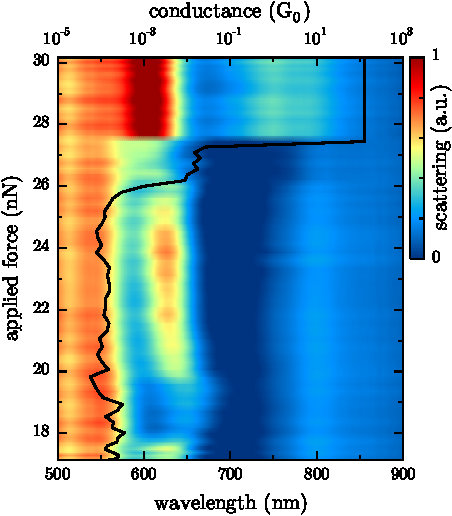
\includegraphics{figures/orig_spherical_tip_dimer_tunnelling_focus}};
\node [above right] at (0,0) {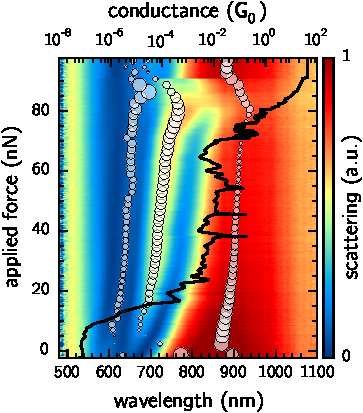
\includegraphics{figures/spherical_tip_dimer_1_tunnelling_focus}};
\node [below left] at (0,0) {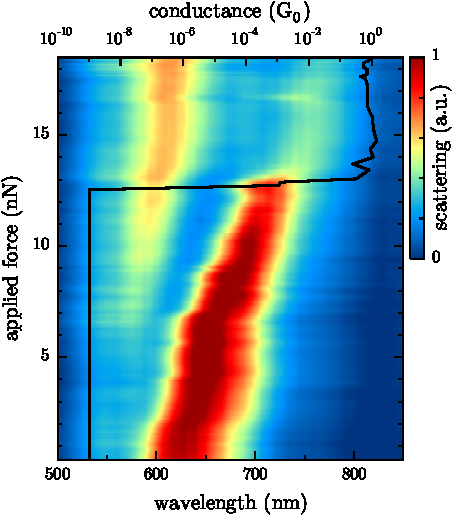
\includegraphics{figures/echem_tip_dimer_tunnelling_focus}};
%\node [below right] at (0,0) {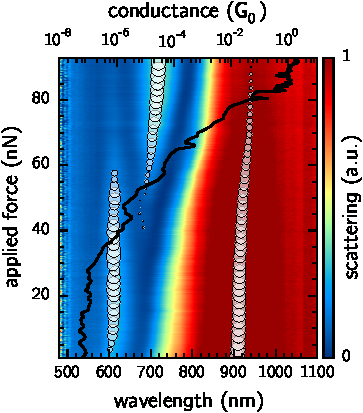
\includegraphics{figures/spherical_tip_dimer_2_tunnelling_focus}};
\node at (-7,7.5) {(a)};
\node at (0.3,7.5) {(b)};
\node at (-7.1,-0.8) {(c)};
%\node at (0.3,-0.8) {(d)};
\end{tikzpicture}
\caption[Scans of multiple spherical tip dimers pushing towards geometrical contact and showing varying phenomena]{\textbf{Scans of multiple spherical tip dimers pushing towards geometrical contact and showing varying phenomena.} Scans show the supercontinuum dark-field scattering spectra as a function of the applied force on the gap with the simultaneously measured conductance superimposed over the axis. The circles highlight the position an evenly distributed selection of the peak position. The size of the circle indicates the amplitude of the mode in the fitted model. Scans a,c and d use Au-coated NanoTools B150 spherical AFM probes to form a dimer while scan b uses electrochemically-fabricated AuNP-on-Pt AFM tips.}
\label{fig:spherical_tip_scans}
\end{figure}

\autoref{fig:spherical_tip_scans} shows a selection of spherical Au tip dimer measurements showing both optical and electronic behaviour once in the sub-nm regime. Simultaneous quantum tunnelling and SDF scattering measurements are presented as a function of the applied force on the gap. Each of the measurements exhibits the signatures of a transition between hybridised and charge transfer plasmons. Interestingly, each scan in the sub-nm regime manages to appear different, at times exhibiting different phenomena related to charge transfer while in the sub-nm regime, regardless of any similar agreement between scans in previous coupling regimes. These differences are thought to originate from surface roughness of even smaller differences in sub-nm scale morphology that affect the way optics and electronics couple. Correctly interpreting and understanding these results is of general importance within the current plasmonics community as smaller gaps begin to become experimentally attainable and the blending of plasmonics and molecular electronics becomes commonplace. Before attempting to unify an explanation between all measurements, each set of measurements is initially considered individually.

\begin{figure}[bt]
\centering
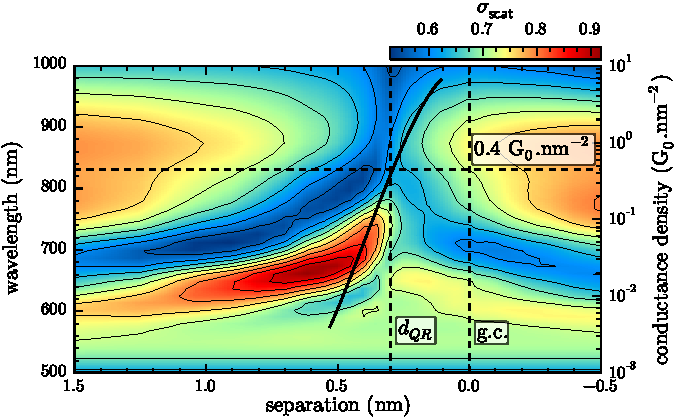
\includegraphics{figures/qcm_tip_theory_zoom}
\caption[Select view of calculated QCM spectra of a spherical tip dimer as a function of separation \cite{savage2012}]{\textbf{Select view of calculated QCM spectra of a spherical tip dimer as a function of separation \cite{savage2012}.} Simulated spectra show that the higher order mode disappears and a CTP mode rises prior to geometrical contact at $d_{QR}=\SI{0.3}{nm}$, prior to geometrical contact (g.c.). This occurs since coherent electron tunnelling transfers enough charge within half an optical cycle to screen hybridised plasmons and eventually excite a CTP. Based on DFT calculations the CTP is excited when the conductance density is \SI{0.4}{G_0.nm^{-2}}.}
\label{fig:qcm_tip_theory}
\end{figure}

Both \autoref{fig:spherical_tip_scans}a and b bear the closest resemblance to the original simulated QCM spectra of sub-nm gaps between spherical Au tips (replotted in \autoref{fig:qcm_tip_theory} with the DFT-calculated conductance density overlaid) \cite{savage2012}, showing the screening of hybridised plasmons and the emergence of CTPs. Screening is indicated by a reduction in the rate of redshift and a decrease in intensity, followed by a blueshift and the formation of new CTP modes to signify the rise of stronger interparticle currents. In theory, these critical currents occur at a conductance density of \SI{0.4}{G_0.nm^{-2}}, at which point two CTPs emerge and hybridised modes disappear. Blueshifts in experimental data appear in similar spectral positions and are therefore similarly attributed to the excitation of CTPs. The fundamental CTP is not measurable using the current microscope as it exists outside of the wavelength range of the spectrometers. The neck of the tip may also act as a short for this mode, preventing it from appearing at all. The behaviour of hybridised modes and higher order CTPs is thus used to interpret the behaviour in the gap.

In both experimental cases, the redshift of each hybridised modes becomes stunted once the conductance rises above $\sim$\num{e-3}\G0, indicating the onset of screening. This is the first critical conductance, revealing the point at which electron tunnelling has risen enough to effectively begin screening gap coupling. The point of blueshift is less clear in \autoref{fig:spherical_tip_scans}a due to the fast transition into geometrical contact. This jump is experienced in almost all scans once the electrostatic pull of the tips is large enough to overcome the meniscus forces holding surfaces apart. \autoref{fig:spherical_tip_scans}b provides a much clearer insight into the origins of the blueshift, and is likely the single most informative scan in terms of demonstrating both screening and blueshifting of plasmons and in agreeing with current theoretical models \cite{zuloaga2009, savage2012}. Its tip approach is much more carefully controlled into geometrical contact, with many measurements in the tunnelling regime and clear observation of discretely quantised conductance channels. It is at this transition between tunnelling and one-dimensional conduction, at around 2\G0, that the blueshift begins to occur and tips enter the quantum conductive regime.

\begin{figure}[bt]
\centering
\begin{tikzpicture}
\node [below left] at (0,0) {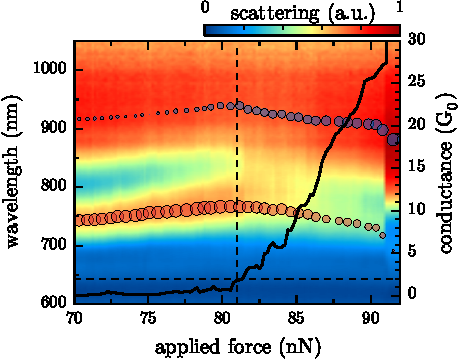
\includegraphics{figures/spherical_tip_dimer_1_tunnelling_focus2}};
\node [below right] at (0,-0.6) {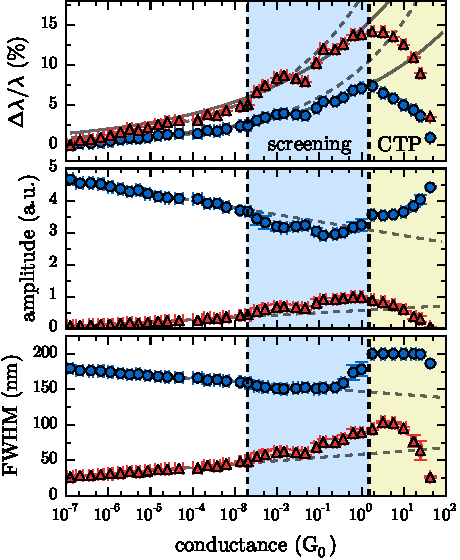
\includegraphics{figures/spherical_tip_dimer_1_tunnelling_analysis}};
\node [below left] at (-7.35,-0.5) {(a)};
\node [below right] at (0,-0.5) {(b)};
\end{tikzpicture}
\caption[Detailed analysis of a spherical Au tip dimer scan in the quantum charge transfer regime]{\textbf{Detailed analysis of a spherical Au tip dimer scan in the quantum charge transfer regime.} The scan shown in \autoref{fig:spherical_tip_scans}b is replotted in (a) with a linear conductance scale to show quantised conductance stepping and its relationship with scattering spectra. Dashed lines indicate the point of blueshift at $G=2\G0$. Peak positions in the fitted model are denoted by circles superimposed onto spectra with their size corresponding to the peak amplitude. The relative shift of each mode from fitted parameters, along with a normalised amplitude, is plotted in (b). Vertical dashed lines highlight the transitions into the tunnelling (crossover) regime at \num{2e-3}\G0 and the conductive regime at 2\G0. Exponential curves are fitted to the wavelength shift for $G<\num{e-3}\G0$ (dashed) and $G>\num{e-3}\G0$ (solid) to highlight the reduction in redshift caused by passing through the screening (tunnelling) threshold. Similar lines are plotting to show the increased amplitude screening upon passing through \num{2e-3}\G0.}
\label{fig:scan3_analysis}
\vspace{-5pt}
\end{figure}

A better view of this transition is shown in \autoref{fig:scan3_analysis}a where the scan shown in \autoref{fig:spherical_tip_scans}b is replotted with a linear conductance scale in order to closer inspect charge transfer behaviour. The turning point in the redshift of both hybridised plasmons initially appears to be at 2\G0 in spectra. Fitting the spectra and extracting the behaviour of each individual mode provides a more quantitative analysis. The results of the fit are superimposed onto spectra in \autoref{fig:scan3_analysis}a with relative peak shifts and mode amplitudes shown separately in \autoref{fig:scan3_analysis}b. Mode positions follow an exponential model as expected. At \num{2e-3}\G0 the redshift deviates from this model and becomes less pronounced. Prior to this point the amplitude of the lower order mode is decreasing due to increasing charge localisation. Upon passing through the first critical conductance at \num{2e-3}\G0 the amplitude is further screened and decreases faster. The higher order mode seemingly gains some intensity at this point, potentially from redistributed charge of the lowest order mode.

The second critical conductance can be defined as 2\G0, a surprisingly appropriate quantity given that it occurs just above the transition from tunnelling into a quantum conductive regime. Upon surpassing 2\G0 the resonance position of both hybridised plasmons begins to strongly blueshift as current passes through the junction, quickly returning to their initial resonance position prior to entering the tunnelling regime. The fitting algorithm is programmed to use the fit of the previous spectrum as an initial guess when fitting the following spectrum. The algorithm computes that the lowest order mode blueshifts into the observed CTP, with an increasing intensity once $G>10\G0$, while the higher order plasmon attenuates into only a weak, blueshifted resonance. %This behaviour, whilst agreeing with previous observations \cite{savage2012}, disagrees with some principles, such as a hybridised modes corresponding CTP should appear far shifted to the IR \cite{romero2006}.
This CTP becomes fully developed during the final pull into geometrical contact. A third critical conductance for CTP development can then be estimated to be around 10\G0 with full development between 30--40\G0.

Despite integer quantised conductance steps being observed in this conductive regime, there is no obvious step-wise behaviour in the optics. Given that it is the charge transfer that leads to the blueshift of hybridised modes it would be intuitive to expect quantised current changes to discretise incremental blueshifts. This is not obviously the case, with the blueshift appearing smooth throughout. More experimental data would be needed to properly understand this observation.

%\begin{figure}[bt]
%\centering
%\def\svgwidth{0.55\textwidth}
%\fontsize{10pt}{1em}\selectfont\subimport{./figures/}{coupled_to_ctp_transition.pdf_tex}
%\caption[]{}
%\label{fig:coupled_to_ctp_transition}
%\vspace{-5pt}
%\end{figure}

Both sets of measurements at the focus of this discussion are not without their issues, however, when comparing with both theory and previous experimental results. \autoref{fig:spherical_tip_scans}a shows variations in both the position and intensity of the \SI{600}{nm} mode, which are attributed to changes in the torsional force on the gap, corresponding to a rotational motion of the tip. The intensities of the final two modes when in contact are also reversed compared with QCM predictions. \autoref{fig:spherical_tip_scans}b looks remarkably closer to theory prior to geometrical contact but deviates when lacking the higher order contact mode at \SI{600}{nm}. Changes in CTP position and intensity are said to originate from the touching profile of the dimer, indicating that the surface roughness may play a role with such large dimer surfaces \cite{zuloaga2009}. This becomes the case since the charge distribution of a bonding hybridised mode is most similar to the charge distribution of the next highest order CTP mode, hence why the CTP appears to emerge from the blueshifting coupled mode.

\begin{figure}[bt]
\centering
\begin{tikzpicture}
\node [below left] at (0,0) {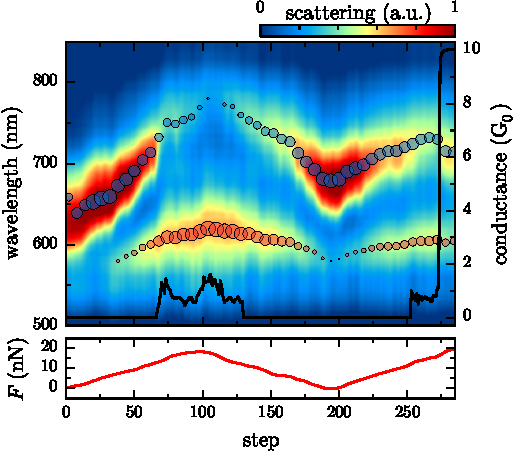
\includegraphics[width=8cm]{figures/echem_tip_dimer_tunnelling_focus_2}};
\node [below right] at (0,-0.2) {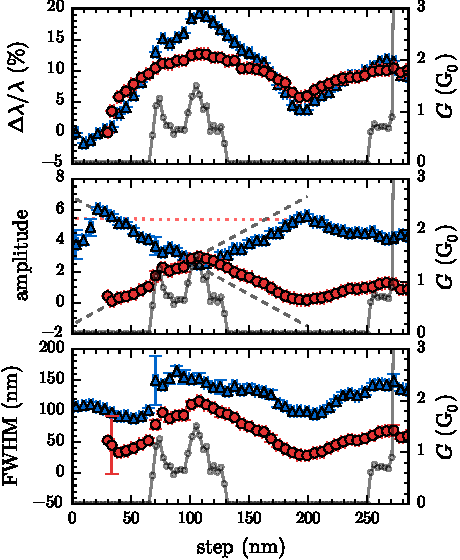
\includegraphics{figures/echem_tip_dimer_tunnelling_analysis}};
\node [below left] at (-7.3,-0.2) {(a)};
\node [below right] at (0,-0.2) {(b)};
\end{tikzpicture}
\caption[Detailed analysis of the extended electrochemically-fabricated spherical AuNP-on-Pt tip dimer scan]{\textbf{Detailed analysis of the extended electrochemically-fabricated spherical AuNP-on-Pt tip dimer scan.}
An extended plot of the  scan shown in \autoref{fig:spherical_tip_scans}c is plotted in (a), demonstrating reproducibility in approaches. The applied force trace represents the separation changes between tips, with tips approached, retracted and then finally approached into geometrical contact. Peak positions in the fitted model are denoted by circles superimposed onto spectra with their size corresponding to the peak amplitude. The relative shift of each mode from fitted parameters, along with a normalised amplitude, is plotted in (b). Linear rates of amplitude variation are revealed from peak fits, removing the width contribution from the peak intensity. Reduced rates of redshift are found in the $G.\G0$ regions with a discontinuous blueshift seen after the $G>2\G0$ transition.}
\label{fig:echem_tip_dimer_analysis}
\end{figure}

\autoref{fig:spherical_tip_scans}c shows a somewhat different phenomena to previous scans, though still in line with quantum transport expectations. Tips in \autoref{fig:spherical_tip_scans}c are highly asymmetric AuNP-on-Pt tips, smoothed using piranha solution. Both have \SI{40}{N.m^{-1}} cantilever spring constants and therefore the force resolution during approach is limited. Prior to tunnelling a higher order mode begins to emerge. The transition into contact is quick, with few to no point at any given conductance, ending initially with a stable 0.75--1.5\G0 contact. In this system, this level of conductance can only be achieved if the junction is rapidly changing its conductive channel width in order to average over states, or if molecular conduction is involved. Once the conductance has risen the initial SPR quickly diminishes without blueshifting and the higher order SPR gains intensity. The screening here is another example of entering into a tunnelling regime but without sufficient current below 2\G0 to excite a CTP and blueshift existing SPRs.

After the initial conductance increase, the tip is then retracted to test for reproducibility, as shown in the extended scan plot in \autoref{fig:echem_tip_dimer_analysis}a. A second approach soon after demonstrates the same phenomenon until the conductance rises above 2\G0 when both modes blueshift. Changes in the redshift and amplitude gradient show the effects of surface roughness as retraction introduces a small degree of misalignment between tips such that the point of closest contact in the second approach is different from the first.

A detailed mode analysis of the SPR positions and amplitudes is found in \autoref{fig:echem_tip_dimer_analysis}, in which the trends described for previous measurements still apply. The peak position behaves as expected. Upon increasing the conductance up to the 1\G0 level there is a visible kink in the redshift as its rate reduces as a result of screening. Once the conductance rises above 2\G0 in the second approach there is a clear blueshift in the lowest order mode. This is a similar, although more abrupt, measurement of the critical conductance than in previous scans. The amplitude behaviour, extracted from the peak fits and separated from the mode width, is interesting as the amplitude of the initial mode linearly decreases during approach at exactly the same rate of increase as the emerging mode. This equality in the gradients is shown by the dotted red line in the figure indicating the constant sum of the two amplitudes. In a sense, charge is conserved and simply switches to a more favourable mode as the gap width decreases. Conceptually, this could suggest that tunnelling begins to reduce coupling between the lowest order modes first, making higher order coupled modes energetically more favourable

Each of the presented three scans show agreement with recent theoretical concepts that define the influence of quantum transport on plasmon coupling. Critical conductances for entering the tunnelling regime and the quantum conductive regime are observed in each case in the vicinity of 1--\num{2e-3}\G0 and 2\G0, respectively. No observation of CTP excitation has been made leaving the final critical conductance yet to be experimentally measured. This is the first time conductance values have been correlated dynamically with optical spectra. Comparison with previously explored systems shows excellent agreement, supporting the idea of a set of fixed critical conductances. Blueshifts of the BDP, forming the SBDP, begin to be seen in small conductive contacts at conductances of 2\G0 in both theoretical models \cite{perez2010, perez2011} and in AuNPs on a Au mirror separated by a blended SAM of variable conductance \cite{benz2014}. Observation of the same threshold conductance in two very different systems provides strong evidence for the fundamental nature of critical conductances.

Variations in the measured phenomena are highly likely to be the result of surface roughness changing the

Further confirmation of such effects could become possible using 2DEGs, the materials initially used to discover quantised conductivity, and those currently being explored for plasmonics. In the original concept a 2DEG is biased at two ends, gated in the centre and electrically depleted to form a 1D constriction through which ballistic transport occurs \cite{van1988quantized, wharam1988one}. Modern 2DEG systems have been shown to support plasmons in the THz regime \cite{}. Thus by gating a plasmonic 2DEG it could be controllably depleted to pass through both the capacitively coupled and conductive regimes. 

%The final scan, \autoref{fig:spherical_tip_scans}d, does not agree with the other scans or theory. Instead, it shows that as a tunnelling current rises a central mode emerges between two diminishing hybridised modes.

%\subsection{Effects of Surface Morphology on Quantum Charge Transport Effects}

%\begin{figure}[bt]
%\centering
%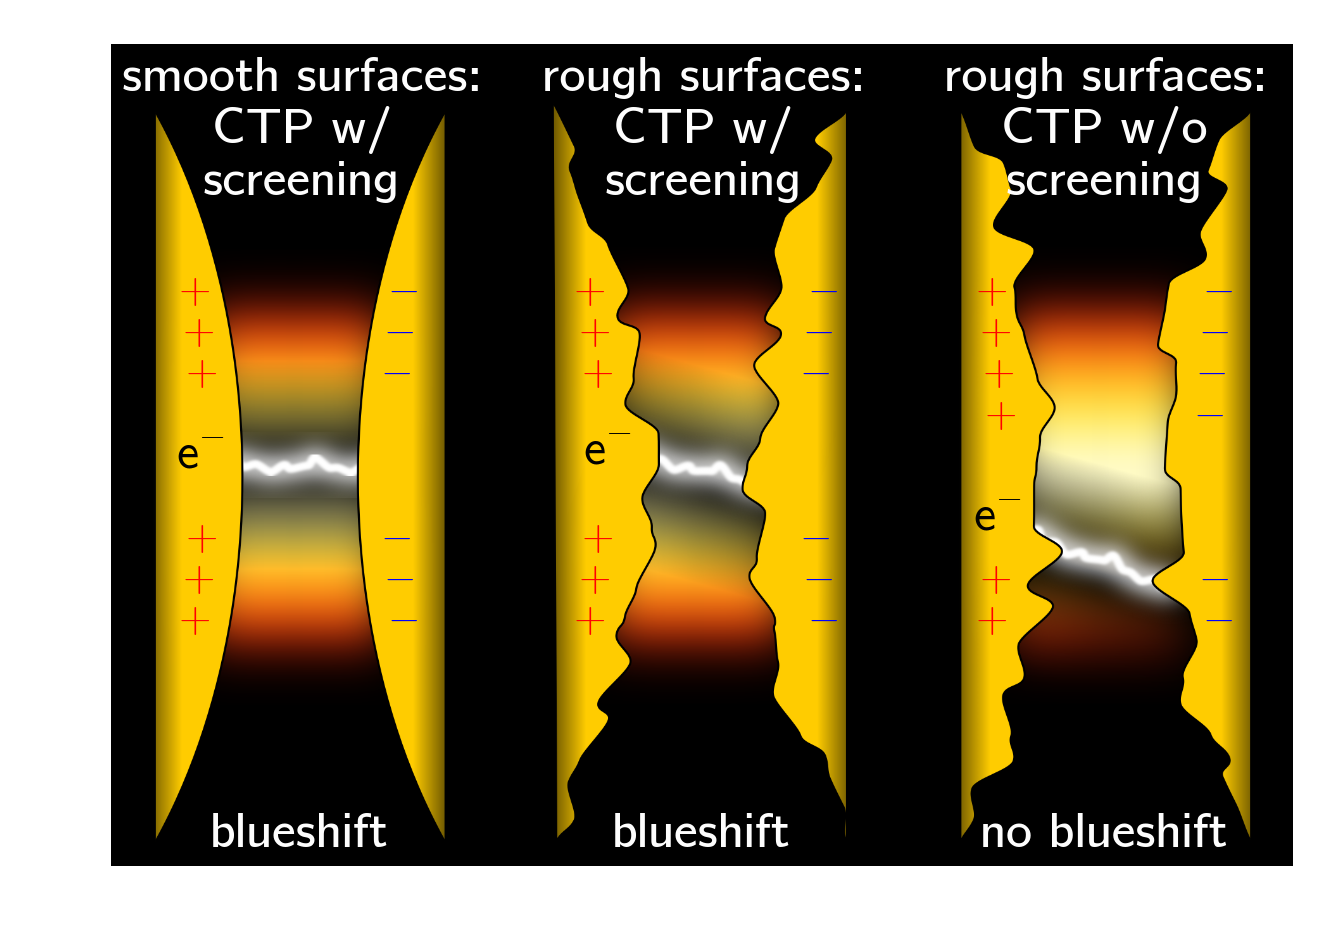
\includegraphics{figures/tunnelling_plasmonics_diagram}
%\caption[Diagram of possible plasmonic gap configurations in the tunnelling regime]{\textbf{Diagram of possible plasmonic gap configurations in the tunnelling regime.} An ideal symmetric dimer surface (a) will have perfect overlap between the plasmon mode and the point tunnelling leading to field screening. Roughened surfaces have a statistically high chance of conforming to the symmetric configuration (b) or the roughness may lead to localisation of the point of tunnelling to outside the plasmonic hotspot (c).}
%\label{fig:tunnelling_plasmonics_diagram}
%\end{figure}

%The hypothesis linking the scans together is that the spatial location of the point or points of conduction in relation to the gap plasmon field is of significant importance. For two ideal (smooth) surfaces coming together the symmetry of the system means that both the gap plasmon field and the shortest conduction path between surfaces are coincident (\figurename~\ref{fig:tunnelling_plasmonics_diagram}a). In this case the optical response is likely to reflect that of QCM spectra \cite{savage2012} (\figurename~\ref{fig:qcm_tip_theory}) with both the emergence of a tunnelling CTP and the gap plasmon modes being screening, and therefore blueshifting, with the increase in tunnelling current.
%For a more realistic surface that includes atomic to nanoscale roughness there is statistically a good chance that the plasmon field and the shortest conduction path {\color{red}overlap/align} (\figurename~\ref{fig:tunnelling_plasmonics_diagram}b). The physics in this case, to a certain extent, retains the characteristics of the QCM model. It is possible that roughness further localises the gap plasmon in places leading to an inhomogeneous plasmon field but these locations would also likely incur a larger tunnelling current.

%Discrepancies between the QCM model and the experimental data occur if the point of conduction does not overlap well with the plasmon field, in which case the field is not screened (\figurename~\ref{fig:tunnelling_plasmonics_diagram}c). The argument that the plasmon field localises most strongly around the region of smallest gap only extends so far as the plasmon will still be more distributed than the conduction path.%
%\footnote{$w_{gLSP}=\sqrt{Rd}$ for a gap plasmon and $w_{c}\propto R$ for conduction, hence the gap plasmon is more laterally distributed.}
%There is a finite plasmonic density of states, however, and so an electron may either accumulate at the metal/gap interface or tunnel across the gap as part of the tunnelling CTP. Under these conditions it is expected that the number of electrons in the CTP mode increases with the d.c. tunnelling current as the gap barrier width decreases. The number of electrons remaining in the coupled mode must then decrease at the same rate to conserve the number of electrons in the overall structure. Under these circumstances only the intensity of the coupled mode is required to decrease. There is no mechanism which necessitates the screening and blueshifting of the coupled modes.
%Furthermore, for the case where the tunnelling results in plasmon screening, there is no reason that the mode amplitude should be conserved during the transition between coupled and CTP modes. Even though the charge must be conserved the contribution of the reduction in coupling to the mode amplitude is entangled with the transfer of charge between plasmon states.

% Summary
To summarise, charge transfer in systems of coupled plasmons exhibit three distinct regimes of interactions. For small conductances characteristic of electron tunnelling (1--\num{2e-3}\G0) coupling begins to be screened by the tunnelling field and the rate of redshift is steadily reduced. Upon passing through the second critical conductance at 2\G0, also known as $G_{BDP}$ in the literature, the hybridised modes blueshift due to increased screening from conductive charge flow in the gap. At this point the gap behaves as a 1D constriction subject to Landauer ballistic quantised conduction. The final conductance threshold, that for CTP excitation, has not yet been determined but instead roughly estimated to be around 30--40\G0 from final conductance values of geometrically contacted gap surfaces. To restate the significance of this work, this is the first time these critical conductance thresholds have been measured in a dynamic dimer system through correlations between simultaneously measured optics and electronics. Using this information, the performance of a sub-nm plasmon system can begin to be characterised and quantified based upon which regime it falls under.

%\emph{How do results compare with theory when using high powers like a Fianium? Compare to \cite{marinica2012}. Could this apply to 2DEG plasmons?}

\end{document}